% !TeX spellcheck = en_US
\documentclass[a4paper,12pt]{article}
\usepackage[utf8x]{inputenc}
\usepackage{wrapfig}
\usepackage{graphicx}
\usepackage{float}
\usepackage{listings}
\usepackage{amsmath}
\usepackage{caption}
\usepackage{subcaption}
\usepackage[usenames,dvipsnames,svgnames,table]{xcolor}

% Title Page
\title{AST2210 - Lab exercise: Diffraction}
\author{Andreas Ellewsen}

\begin{document}
\maketitle
%\tableofcontents

\section{Diffraction by a single slit}
\subsection{Setup}
For this exercise, we will use a simple set-up with a small laser and a 100 µm slit. The small laser tube is mounted  on a simple platform and powered by a 4.5V flat battery. The laser is aimed at the slit, and the diffraction pattern is projected on the wall.
\subsection{Exercises}
First we want to measure the wavelength of the laser by using the diffraction $asin(\theta) = m\lambda$, where $a$ is the width of the slit, and $m$ the order of the minimum. Combing basic trigonometry and the above formula gives $m\lambda = \frac{ap}{d}$, where $p$ is the distance between the minimums on the wall, and $d$ is the distance from the slit to the wall. \\
Solving for $\lambda$: 
\begin{equation}
\lambda = \frac{ap}{md}
\label{eq1}
\end{equation}
In the lab we measured that the distance between order -3 to +3 was 6.2 $\pm$ 0.1 cm. Taking the average of this gives $p = 1.033.. \pm 0.166..$cm, and $d = 133.5 \pm 1 $cm.
If we then set $m = 1$ and put the rest of the numbers into equation (1) we get that $\lambda = 774.26 \pm 36.6$ nm, which sound like a reasonable answer.

When this is done, we replace the slit by an "anti-slit", in this case a paper clip. Looking at the diffraction pattern now reveals that we are seeing the inverse of what we saw with the slit.
When considering Babinet's principle this is as expected. The reason this happens is because all we've done different from the slit experiment is to change the surface the laser has to pass through. And this change is the inverse of the slit. In simpler words; it's opaque where the slit is transparent, and transparent where the slit is opaque. Thus we can use the same equations as have already been used. The width of the paper clip can then be found using
\begin{equation}
a = \frac{\lambda md}{p}
\end{equation}

Setting $m=1$, $d=206.5 \pm 2$ cm. The distance between order 0 and 30 is found to be $4.5 \pm 0.1 cm$. Taking the average of this gives $p = 0.75 \pm 0,01666..$. Inserting these numbers and the wavelength found for the laser into equation (2) gives a thickness of $a = 1.0684 \pm 0.0846$ mm, which also seems to be reasonable.

\section{Diffraction by a circular aperture}
\subsection{Setup}
For this exercise, we will use a set-up with the laser connected through the fiber to the collimator tube, with dampening filter. The (parallel) light from the tube is focused by an f=100 mm doublet lens. The microscope objective and mono-chromatic camera are used to magnify and image the Airy pattern in the focal plane.

\subsection{Exercises}
First we verify that the microscope objective correctly images the focal plane. We were supposed to record an exposure of this, but for some reason we didn't. Because of this we can assume that the image is in focus, and we can thus assume the distance between the objective and lens to be $D = 10$ cm, since the focal length of the lens is 10 cm.

The angle of the minima is given by the formula $sin(\theta) = K\lambda/d$, where $d=5 \pm 0.1$cm is the diameter of the aperture. For the first minimum, the constant K = 1.22. 

We take an exposure of this, which can be seen in figure \ref{fig:airy}. 
Using this image, one can calculate the values for K for the second and third minima. 
We do this be first counting that the first minima is 5 pixels from the center, the second minima is 11 pixels from the center, and the third minima is 16 pixels from the center.
Remembering the 20 times magnification of the objective and the pixelsize of 6µm for the camera, we need to multiply the values in pixels by $6 \text{µm/pixel}$, and divide by $20$ because of the magnification.\\

All of this yields the following equation:
\begin{equation}
r/D = K\lambda/d
\end{equation}
Solving for K gives:
\begin{equation}
K=\frac{rd}{D\lambda}
\end{equation}

Testing for the first minimum gives a fairly wrong answer of $K = 0.97 \pm 0.06$, but at least that way we know that there is a pretty large error in our estimates.

In this case we found that for the second minimum, $K = 2.13 \pm 0.14$ and for the third minimum, $K = 3.10 \pm 0.20$. 

\begin{figure}
	\centering
	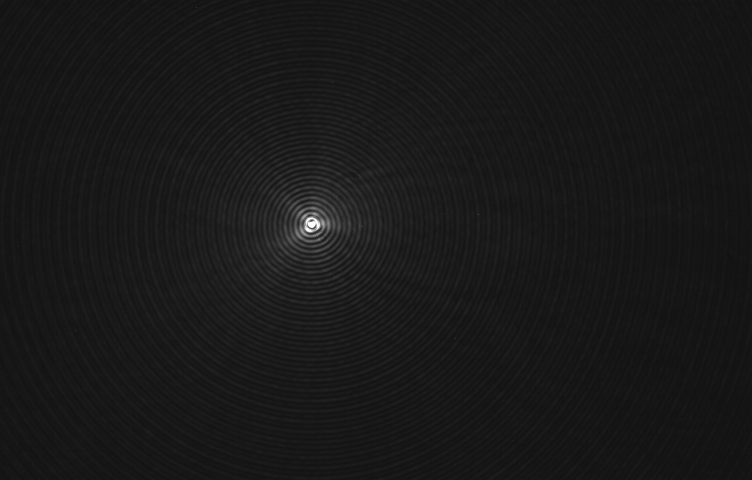
\includegraphics[width=\textwidth]{airy}
	\caption{Single slit}\label{fig:airy}
\end{figure}

Once this was done, we were supposed to use the circular aperture reducer to reduce the aperture and record exposures at different amounts of reduction. For some reason these exposures were not saved. When this was done one could observe that the distance between the rings was reduced, but the number of rings stayed constant with small changes in aperture size. 

After that we took a close look at the patterns of dust in the optical system. An exposure of this should have been saved, but was not. We noticed that the dust particles made their own tiny airy disks, which is to be expected considering Babinet's principle.

To finish we want to look at Arago's spot. To do this we remove the lens from the set-up and replace it by a coin (without a central hole), remove the objective and the camera. The dampening filter is then removed and replaced by the corresponding part of the white light tube. The laser is then turned on and we see the picture recorded in figure \ref{fig:arago}. It really is too bad that the picture is so low quality. When the picture was taken, one could se a tiny red spot in the middle of the dark area. This spot in the dark area is called Arago's spot, and is a result of the wave nature of light. 

\begin{figure}
	\centering
	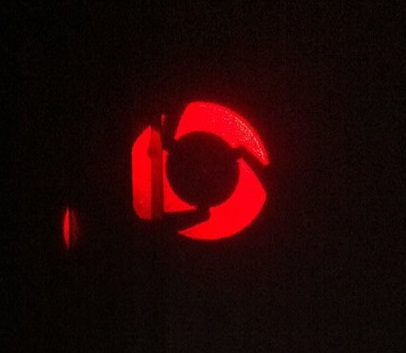
\includegraphics[width=\textwidth]{arago}
	\caption{Arago's spot}\label{fig:arago}
\end{figure}

\section{Summary}
In this lab we've gone through diffraction by a slit, an "anti-slit", and a circular aperture. The answers we got for the slit and the "anti-slit" were reasonable answers. The answer for the first minimum on the circular aperture showed that something was not measured correctly in our setup, but surprisingly, the answers for the second and third minima were pretty accurate. We also observed Arago's spot. In the future there should be done a better job at taking exposures of the things that are observed during the lab.

\end{document}